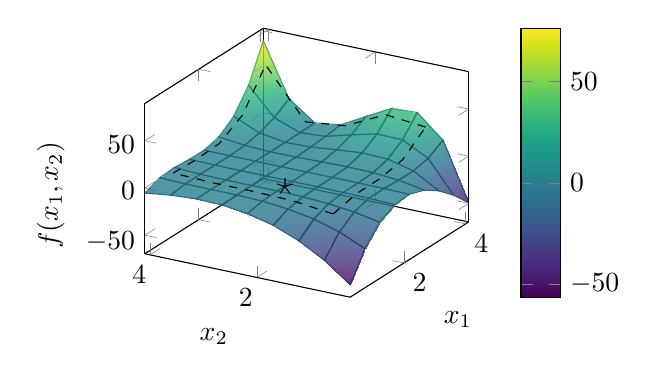
\begin{tikzpicture}
    \begin{axis}[
        view={-60}{30},
        grid=minor,
        colormap/viridis,
        xlabel={$x_1$},
        ylabel={$x_2$},
        zlabel={$f(x_1, x_2)$},
        scale=0.6,
        colorbar,
        domain=0.25:4.1,
        y domain=0.25:4.1,
        samples=9
    ]
        \addplot3[
            surf,
            opacity=0.8,
            shader=faceted interp,
        ] {(x-2)^2*(y-3)^2*(x*y-2.5)};

        %add plot at the optimal solution
        \addplot3[
            mark=star,
            mark size=3,
            only marks,
            mark options={draw=black},
        ] coordinates {(1.438, 2.158, 0.1350)};

        %add lines for the feasible region at function height with intermediate points
        \addplot3[
            mark=none,
            style=dashed,
            color=black,
        ] coordinates {
            (1, 1, {(1-2)^2*(1-3)^2*(1*1-2.5)}) 
            (1.75, 1, {(1.75-2)^2*(1-3)^2*(1.75*1-2.5)})
            (2.5, 1, {(2.5-2)^2*(1-3)^2*(2.5*1-2.5)})
            (3.25, 1, {(3.25-2)^2*(1-3)^2*(3.25*1-2.5)})
            (4, 1, {(4-2)^2*(1-3)^2*(4*1-2.5)})
        };

        \addplot3[
            mark=none,
            style=dashed,
            color=black,
        ] coordinates {
            (1, 4, {(1-2)^2*(4-3)^2*(1*4-2.5)}) 
            (1.75, 4, {(1.75-2)^2*(4-3)^2*(1.75*4-2.5)})
            (2.5, 4, {(2.5-2)^2*(4-3)^2*(2.5*4-2.5)})
            (3.25, 4, {(3.25-2)^2*(4-3)^2*(3.25*4-2.5)})
            (4, 4, {(4-2)^2*(4-3)^2*(4*4-2.5)})
        };

        \addplot3[
            mark=none,
            style=dashed,
            color=black,
        ] coordinates {
            (1, 1, {(1-2)^2*(1-3)^2*(1*1-2.5)}) 
            (1, 1.75, {(1-2)^2*(1.75-3)^2*(1*1.75-2.5)})
            (1, 2.5, {(1-2)^2*(2.5-3)^2*(1*2.5-2.5)})
            (1, 3.25, {(1-2)^2*(3.25-3)^2*(1*3.25-2.5)})
            (1, 4, {(1-2)^2*(4-3)^2*(1*4-2.5)})
        };

        \addplot3[
            mark=none,
            style=dashed,
            color=black,
        ] coordinates {
            (4, 1, {(4-2)^2*(1-3)^2*(4*1-2.5)}) 
            (4, 1.75, {(4-2)^2*(1.75-3)^2*(4*1.75-2.5)})
            (4, 2.5, {(4-2)^2*(2.5-3)^2*(4*2.5-2.5)})
            (4, 3.25, {(4-2)^2*(3.25-3)^2*(4*3.25-2.5)})
            (4, 4, {(4-2)^2*(4-3)^2*(4*4-2.5)})
        };
        
    \end{axis}
\end{tikzpicture}